\documentclass[a4paper]{article}
\usepackage[utf8]{inputenc}
\usepackage{graphicx}
\usepackage{multirow}
\usepackage{fancyhdr}
\usepackage{hyperref}
\pagestyle{fancy}
\begin{document}
\begin{tabular}{p{7cm}r}
\textbf{Michał Radmacher}&\multirow{10}{*}{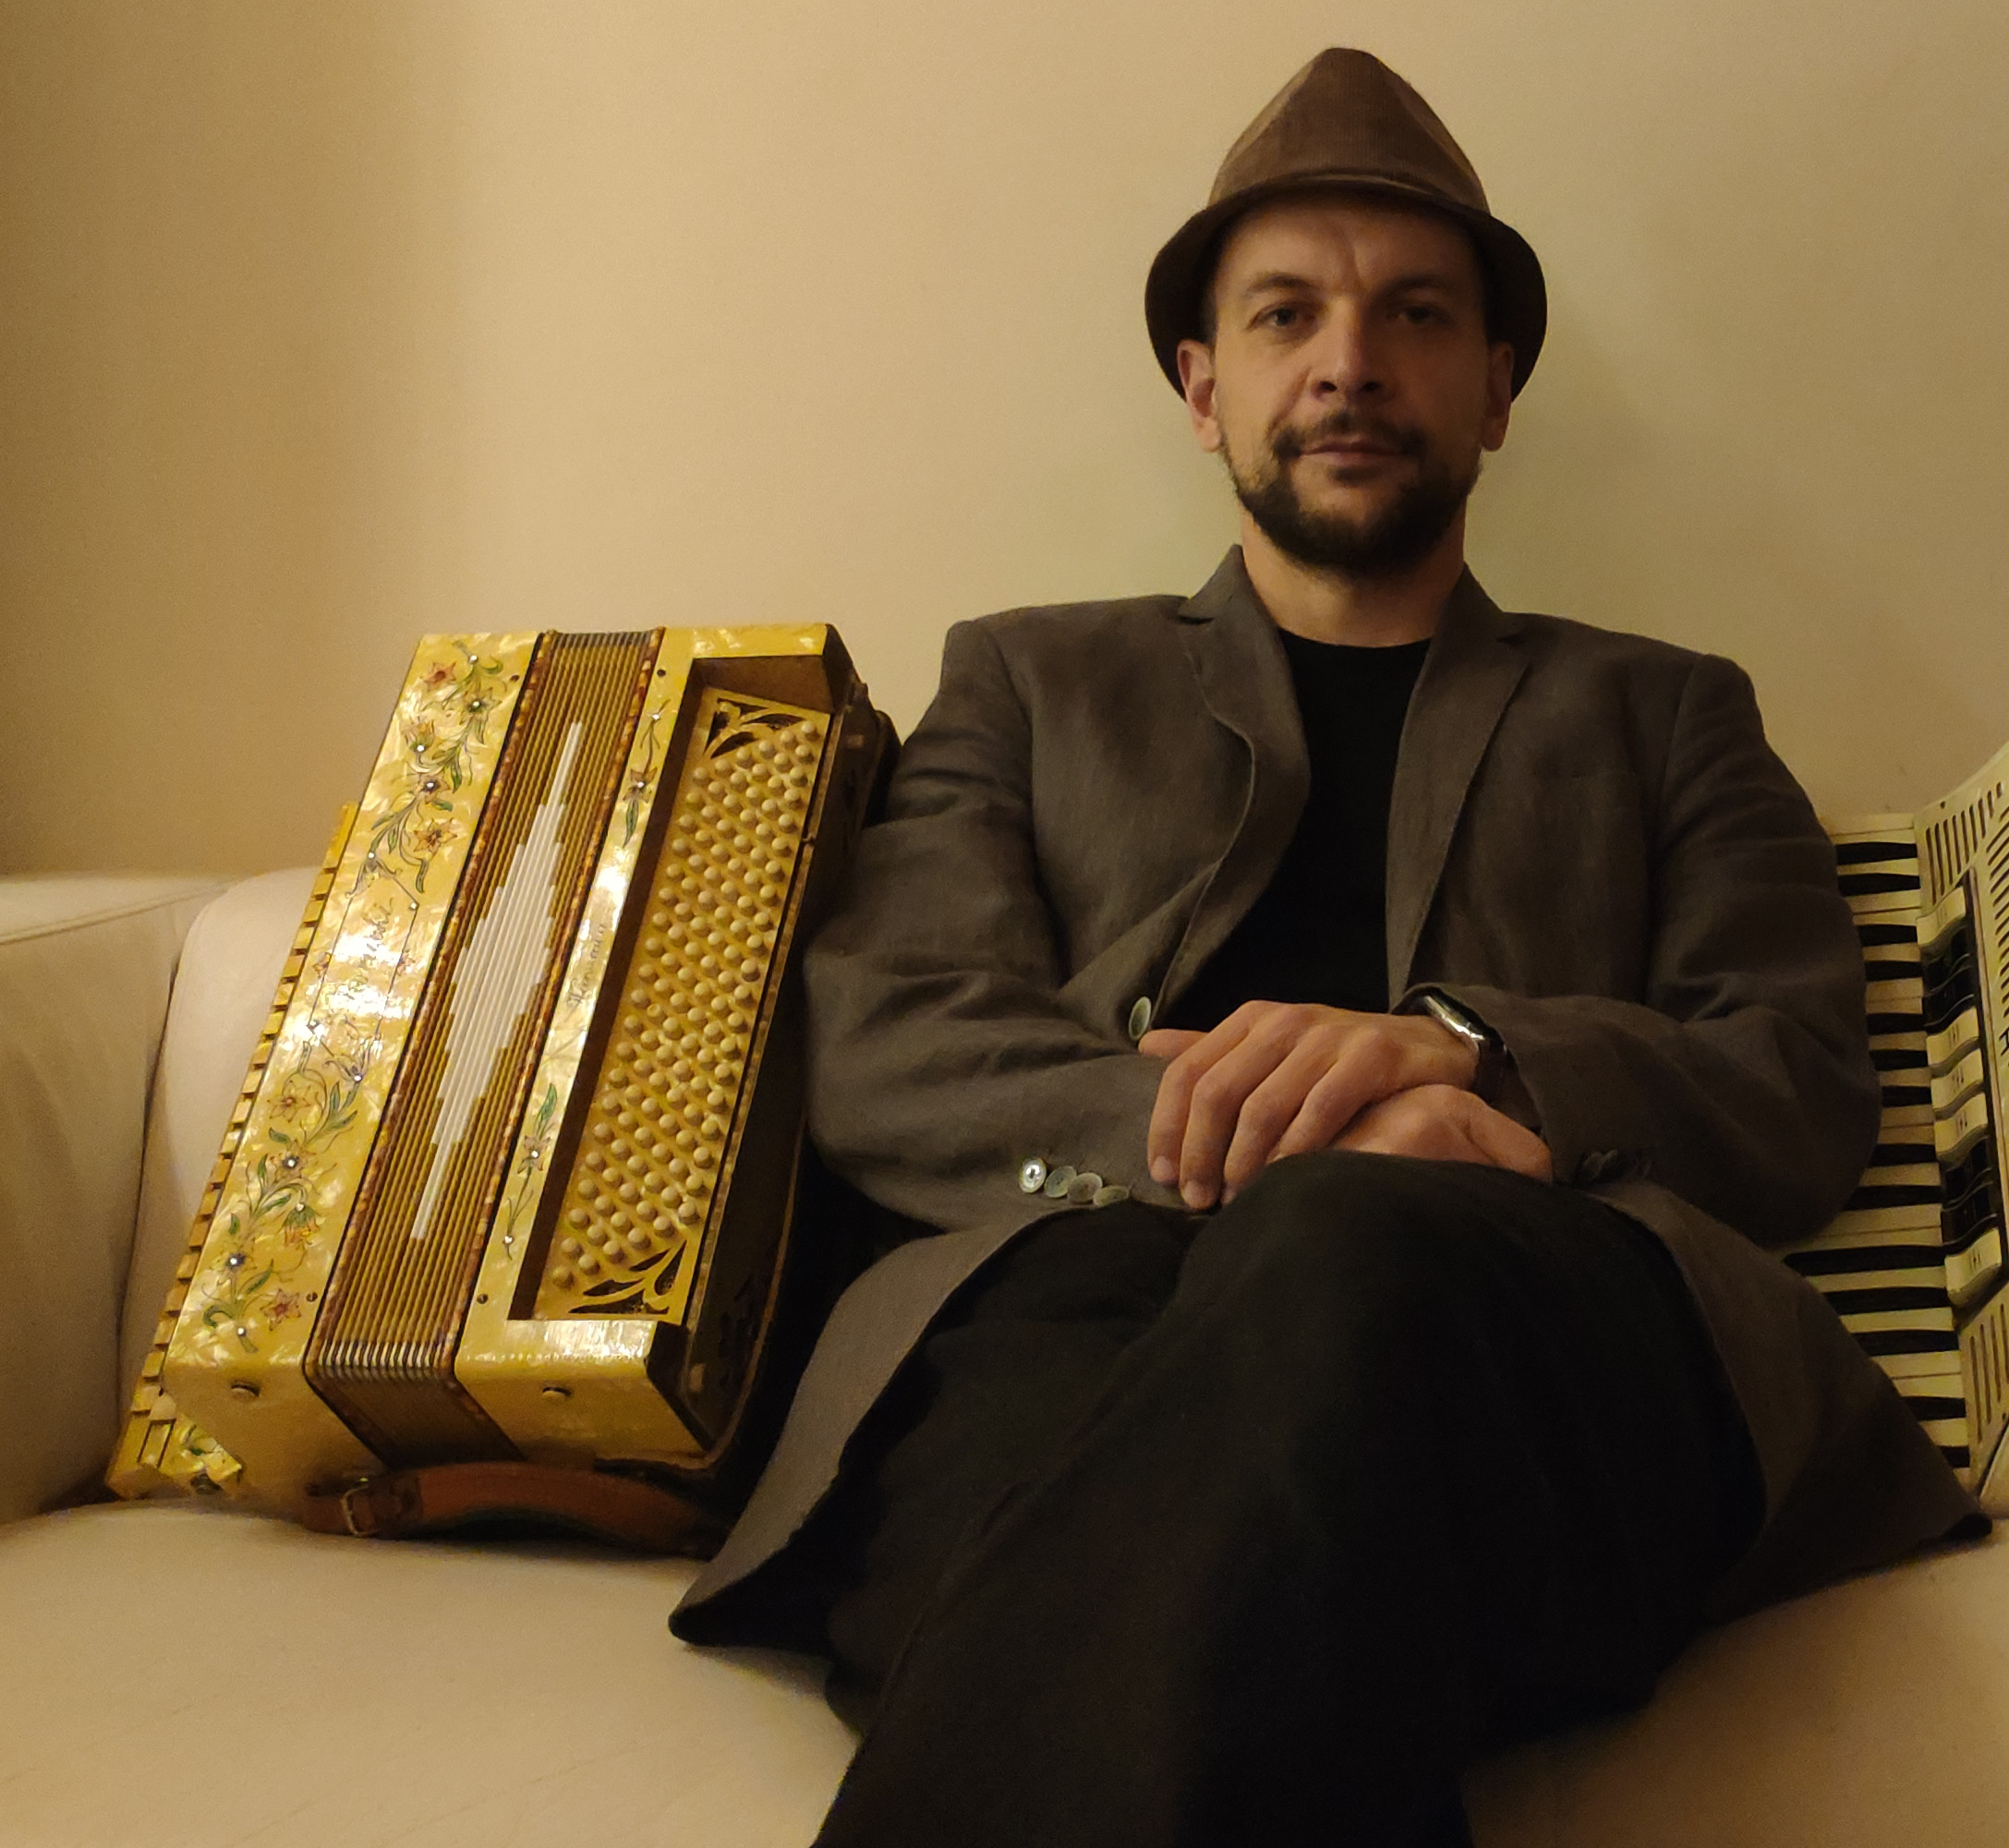
\includegraphics[width=40mm]{mr.jpg}}\\
&\\
\href{https://github.com/mradmacher/}{
\includegraphics{github.png}}\\
&\\
+48 662 974 971&\\
michal@radmacher.pl&\\
&\\
&\\
I like hacking around interesting projects with interesting people.
&\\
&
\end{tabular}

\subsection*{\center{WORK EXPERIENCE}}

\begin{itemize}
  \item
  since 03.2014,
  CipherHealth
  \begin{itemize}
    \item
      working mostly in the backend, developing and maintaining key products for \textbf{healthcare} industry
    \item
      \textbf{Ruby}, MongoDB, PostgreSQL, Cloud technologies
  \end{itemize}
  \item
    09.2012-02.2014,
    Polcode
    \begin{itemize}
      \item
        designing and developing web applications with direct cooperation with \textbf{international customers}
      \item
        \textbf{Ruby on Rails}, PostgreSQL, JavaScript, HTML, CSS
    \end{itemize}
  \item
    02.2010-08.2012,
    Softelnet
    \begin{itemize}
      \item
        maintaining and developing an inventory system
        for one of the leading Polish \textbf{telecom} operators
      \item
        telecommunication, \textbf{PowerBuilder}, \textbf{PL/SQL}, SQL
    \end{itemize}
  \item
    11.2008-01.2010,
    Seihosoft
    \begin{itemize}
      \item
        designing and implementation of \textbf{distributed computer system}
        for a chain of stores
      \item
        \textbf{Java}, JMS, Hibernate
    \end{itemize}
  \item
    Personal projects
    \begin{itemize}
      \item
        \href{https://github.com/mradmacher/paleolog}{PaleoLog} --- web application for biostratigraphers which allows
        to share \textbf{geological} knowledge and helps with micropalaeontological data analysis
      \item
        a couple of websites: \href{https://czarnymotyl.art}{https://czarnymotyl.art} \href{https://balkanartz.eu}{https://balkanartz.eu}, \href{https://karoryfer.com}{https://karoryfer.com}
    \end{itemize}
\end{itemize}

\subsection*{\center{EDUCATION}}
\begin{itemize}
  \item
    10.2005-05.2009 \textbf{Engineer}, School of Banking and Management in Krakow, IT

  \item
    10.2001-05.2005 Incomplete Higher Education,
    \textbf{Jagielonian University in Krakow, Mathematics}

  \item
    1998-2004 \textbf{Musician},
    Second level Musical State School of Władysław Żeleński in Krakow
\end{itemize}

\subsection*{\center{SKILLS}}
\begin{itemize}
\item
  Ruby, JavaScript
\item
  PostgreSQL, MongoDB
\item
  Linux
\item
  GIT
\item
  Vim
\end{itemize}

\subsection*{\center{LANGUAGES}}
\begin{itemize}
\item
  \textbf{Polish} --- native
\item
  \textbf{English}, Spanish, Russian, Bulgarian --- communicative (spoken and written)
\end{itemize}

\subsection*{\center{OTHER INTERESTS}}
\begin{itemize}
\item
	I play clarinet, accordion, kaval and piano. Check out my bands: \href{https://soundcloud.com/czarny-motyl}{Czarny Motyl}, \href{https://soundcloud.com/iglika-pl}{Iglika}, \href{https://soundcloud.com/user-919481466}{BalkanArtz}.
\item
  I learn human and computer languages.
\item
  I practise karate.
\end{itemize}

%\begin{tabular}{p{7cm}r}
%&\\
%&\\
%&\\
%&\\
%&\\
%&\\
%&\\
%&\\
%&\\
%&\\
%&\\
%&\\
%&
%\end{tabular}

%\small{
%I hereby agree for processing the following personal information for recruitment purposes in accordance with
%the regulation regarding the protection o personal data passed on the following date 29.08.97 r. Journal of Laws No 133 pos. 883. }
\end{document}
